\chapter{Background}
\vspace{-1.6em}
\hspace{57pt}{\large\textbf{Contents}}%

\minitoc
\thispagestyle{empty}
\newpage

\section{Altered States of Consciousness}\label{sec:asc_definition}
\textcite{ludwig1966altered} define \acp{ASC} as ,,any mental state(s), induced by various physiological, psychological, or pharmacological maneuvers or agents, which can be recognized subjectively by the individual himself (or by an objective observer of the individual) as representing a sufficient deviation in subjective experience or psychological functioning from certain general norms for that individual during alert, waking consciousness.``

This term is meant to encompass phenomena such as sleep, dream states, day dreaming, hypnosis, sensory deprivation, hysterical states of dissociation and depersonalization, pharmacologically induced mental aberrations and so on, and provide a framework for further analysis of these phenomena.

With regards to psychedelics specifically; \acp{ASC} induced by psychedelics are mainly characterized by profound alterations in sensory perception, mood, thought including the perception of reality, and the sense of self \autocite{preller2016phenomenology}.

\subsection{Phenomenology of Psychedelic States}
The main component of the psychedelic experience is the concept of the \textit{phenomenological ego} and the way it is influenced throughout the experience.


\begin{aquote}{\autocite{preller2016phenomenology}}
    According to \textcite{metzinger2009ego}, the ego is the content of a self-model; this conscious self-model constructed by the brain allows us to interact with our internal world as well as with the external environment in a holistic manner. In a broad sense, the self encompasses features such as a first-person perspective, feelings of agency, ownership (“mineness”) and immediacy (“nowness”), spatial perspective, autobiographical memory, emotions, perceptions, thoughts and acts of will, as well as the feeling of being embedded in our bodily sensations \autocites{metzinger2009ego}{northoff2011self}.

    Another function of the ego serves is to help control and plan our behavior and to understand the behavior of others. By representing the process of representation itself, we can catch ourselves in the act of knowing. Ultimately, the subjective experience of the ego arises from dynamic self-related information processing, which is the result of a self-organizing brain system interacting with its environment, because no such things as selves exist in the world \autocite{metzinger2009ego}.
\end{aquote}

According to \textcite{masters2000varieties}, modified by \textcite{preller2016phenomenology}, the suppression of the \textit{phenomenological ego} during the results in distinctive stages of the psychedelic experience, with alterations at:

\begin{enumerate}
    \setlength{\itemsep}{0pt}
    \setlength{\parskip}{0pt}
    \item The perceptual level: Most frequent and robust features of the psychedelic experience. Perceptual effects are dominated by visual phenomena. Transformation of the environment and alterations of the body image are frequently reported.
    \item The recollective-psychodynamic level: Visual images become more personalized, and boundaries between consciousness and unconsciousness dissolve, causing recall and re-enacting of past experiences and memories and releasing emotions into the process.
    \item The symbolic existential level: More personal involvement and emotional engagement is develop during this stage. Subjects become more personally involved and emotionally engaged as a participant in the ongoing psychedelic scenario.
    \item \textbf{The deep integral level of self-transcendence}: Along with the increasing dissolution of the ego, the psychedelic experience can peak in a state where subjects can become immersed for seconds or minutes in a profound awareness of oneness in which all boundaries disappear and objects are unified into a totality.
\end{enumerate}
\signed{\autocite{preller2016phenomenology}}

The intensity and duration of the psychedelic experience depends most critically on the dosage, the specific drug, and the route of administration. However, other factors, such as personality structure, the nature and dynamics of unconscious material activated, the setting (physical, cultural, and social environment) in which the experience takes place, and the expectancy of the subject are also important \autocite{preller2016phenomenology}. See figure \ref{fig:temporal-dynamics}.

\begin{figure}[H]
    \centering
    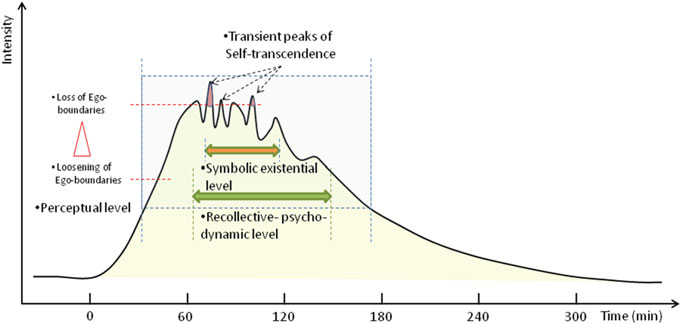
\includegraphics[width=0.95\textwidth]{img/reused/preller2016phenomenology1.png}
    \caption{Temporal dynamics and stages of a psilocybin-induced psychedelic experience. Adaptation by \textcite{preller2016phenomenology} of the original by \textcite{leuner1962experimentelle}.}\label{fig:temporal-dynamics}
\end{figure}

\subsection{Aspects}
For the purpose of this thesis, we define an \textit{aspect} of an \ac{ASC} as a single, distinctive phenomenon of an \ac{ASC}. An \textit{aspect} does not describe the entirety of the \acp{ASC}, only a particular part of it. In order to model \acp{ASC}, we analyze them and break them down into their respective \textit{aspects}.

An example that is common for \acp{ASC} induced by psychedelics is the distortion in the perception of time.

\subsection{Replications}
\textit{Replications} are recreations or simulations of one or more aspects of \acp{ASC} using various forms of media (audio, video, tactile, etc.) with the intention of communicating the experience of \acp{ASC}. Many examples are described in section \ref{sec:introduction}. Various artistic \textit{replications} may be viewed at \textcite{pw2022replications}.

For the rest of this thesis, \textit{a replication} will refer to a recreation or simulation of a \textit{single} aspect of \acp{ASC}. Furthermore, a \textit{complex replication} will refer to a combination of \textit{replications}.

A \textit{replication} of time perception distortion may be simulated via the augmentation of the playback speed of a videoclip using non-linear resampling, or via the augmentation of the simulation speed (timestep) of a \ac{VR} application. This augmentation may be performed by replacing the original sampling function $s \colon \mathbb{R} \to \mathbb{R}$ by $s'(t) = s(t) + f(t)$ where $f \colon \mathbb{R} \to \mathbb{R}$ is a function for sampling procedurally generated noise, such as Perlin noise \autocite{perlin1985image} or Simplex noise \autocite{olano2002simplex}.

\section{Psychometric Evaluation Methods}
Psychometric evaluation of \acp{ASC} are generally performed via questionnaires, of which there are many available.
\textcites{schmidt2018empirische}{figueiredobuilding} performed an analysis of 9 such questionnaires and recommends the \acf{11-ASC} and the \ac{PCI} questionnaires for general assessment of \acp{ASC}.

The \ac{11-ASC} was chosen over the \ac{PCI} due to the popularity of the \ac{11-ASC} in the evaluation of psychedelic-induced \acp{ASC}, and because of the complete lack of \ac{VR}-related studies using the \ac{11-ASC}.

A czech translation of the \ac{11-ASC} was used. The translation was kindly provided by the developers of the \textit{iTrip} smartphone application \autocite{nimh2020itrip}, developed by \fref{https://web.archive.org/web/20220504111203/https://psyres.eu/}{PSYRES} (a czech foundation for psychedelic research) in partnership with \fref{https://web.archive.org/web/20220504110718/https://czeps.org/}{CZEPS} (Czech Psychedelic Society), and was corrected for spelling mistakes and formatting consistency. Unfortunately, we are not aware of any czech translation that has been statistically validated, and for the purpose of this thesis, we assume the used translation (see appendix \ref{appendix:questionnaire}) is statistically valid.
